\subsection{Comparing human and agent scores on every probe task}
\label{app:human-scale-adaptation}

\begin{figure}[h!]
    \centering
    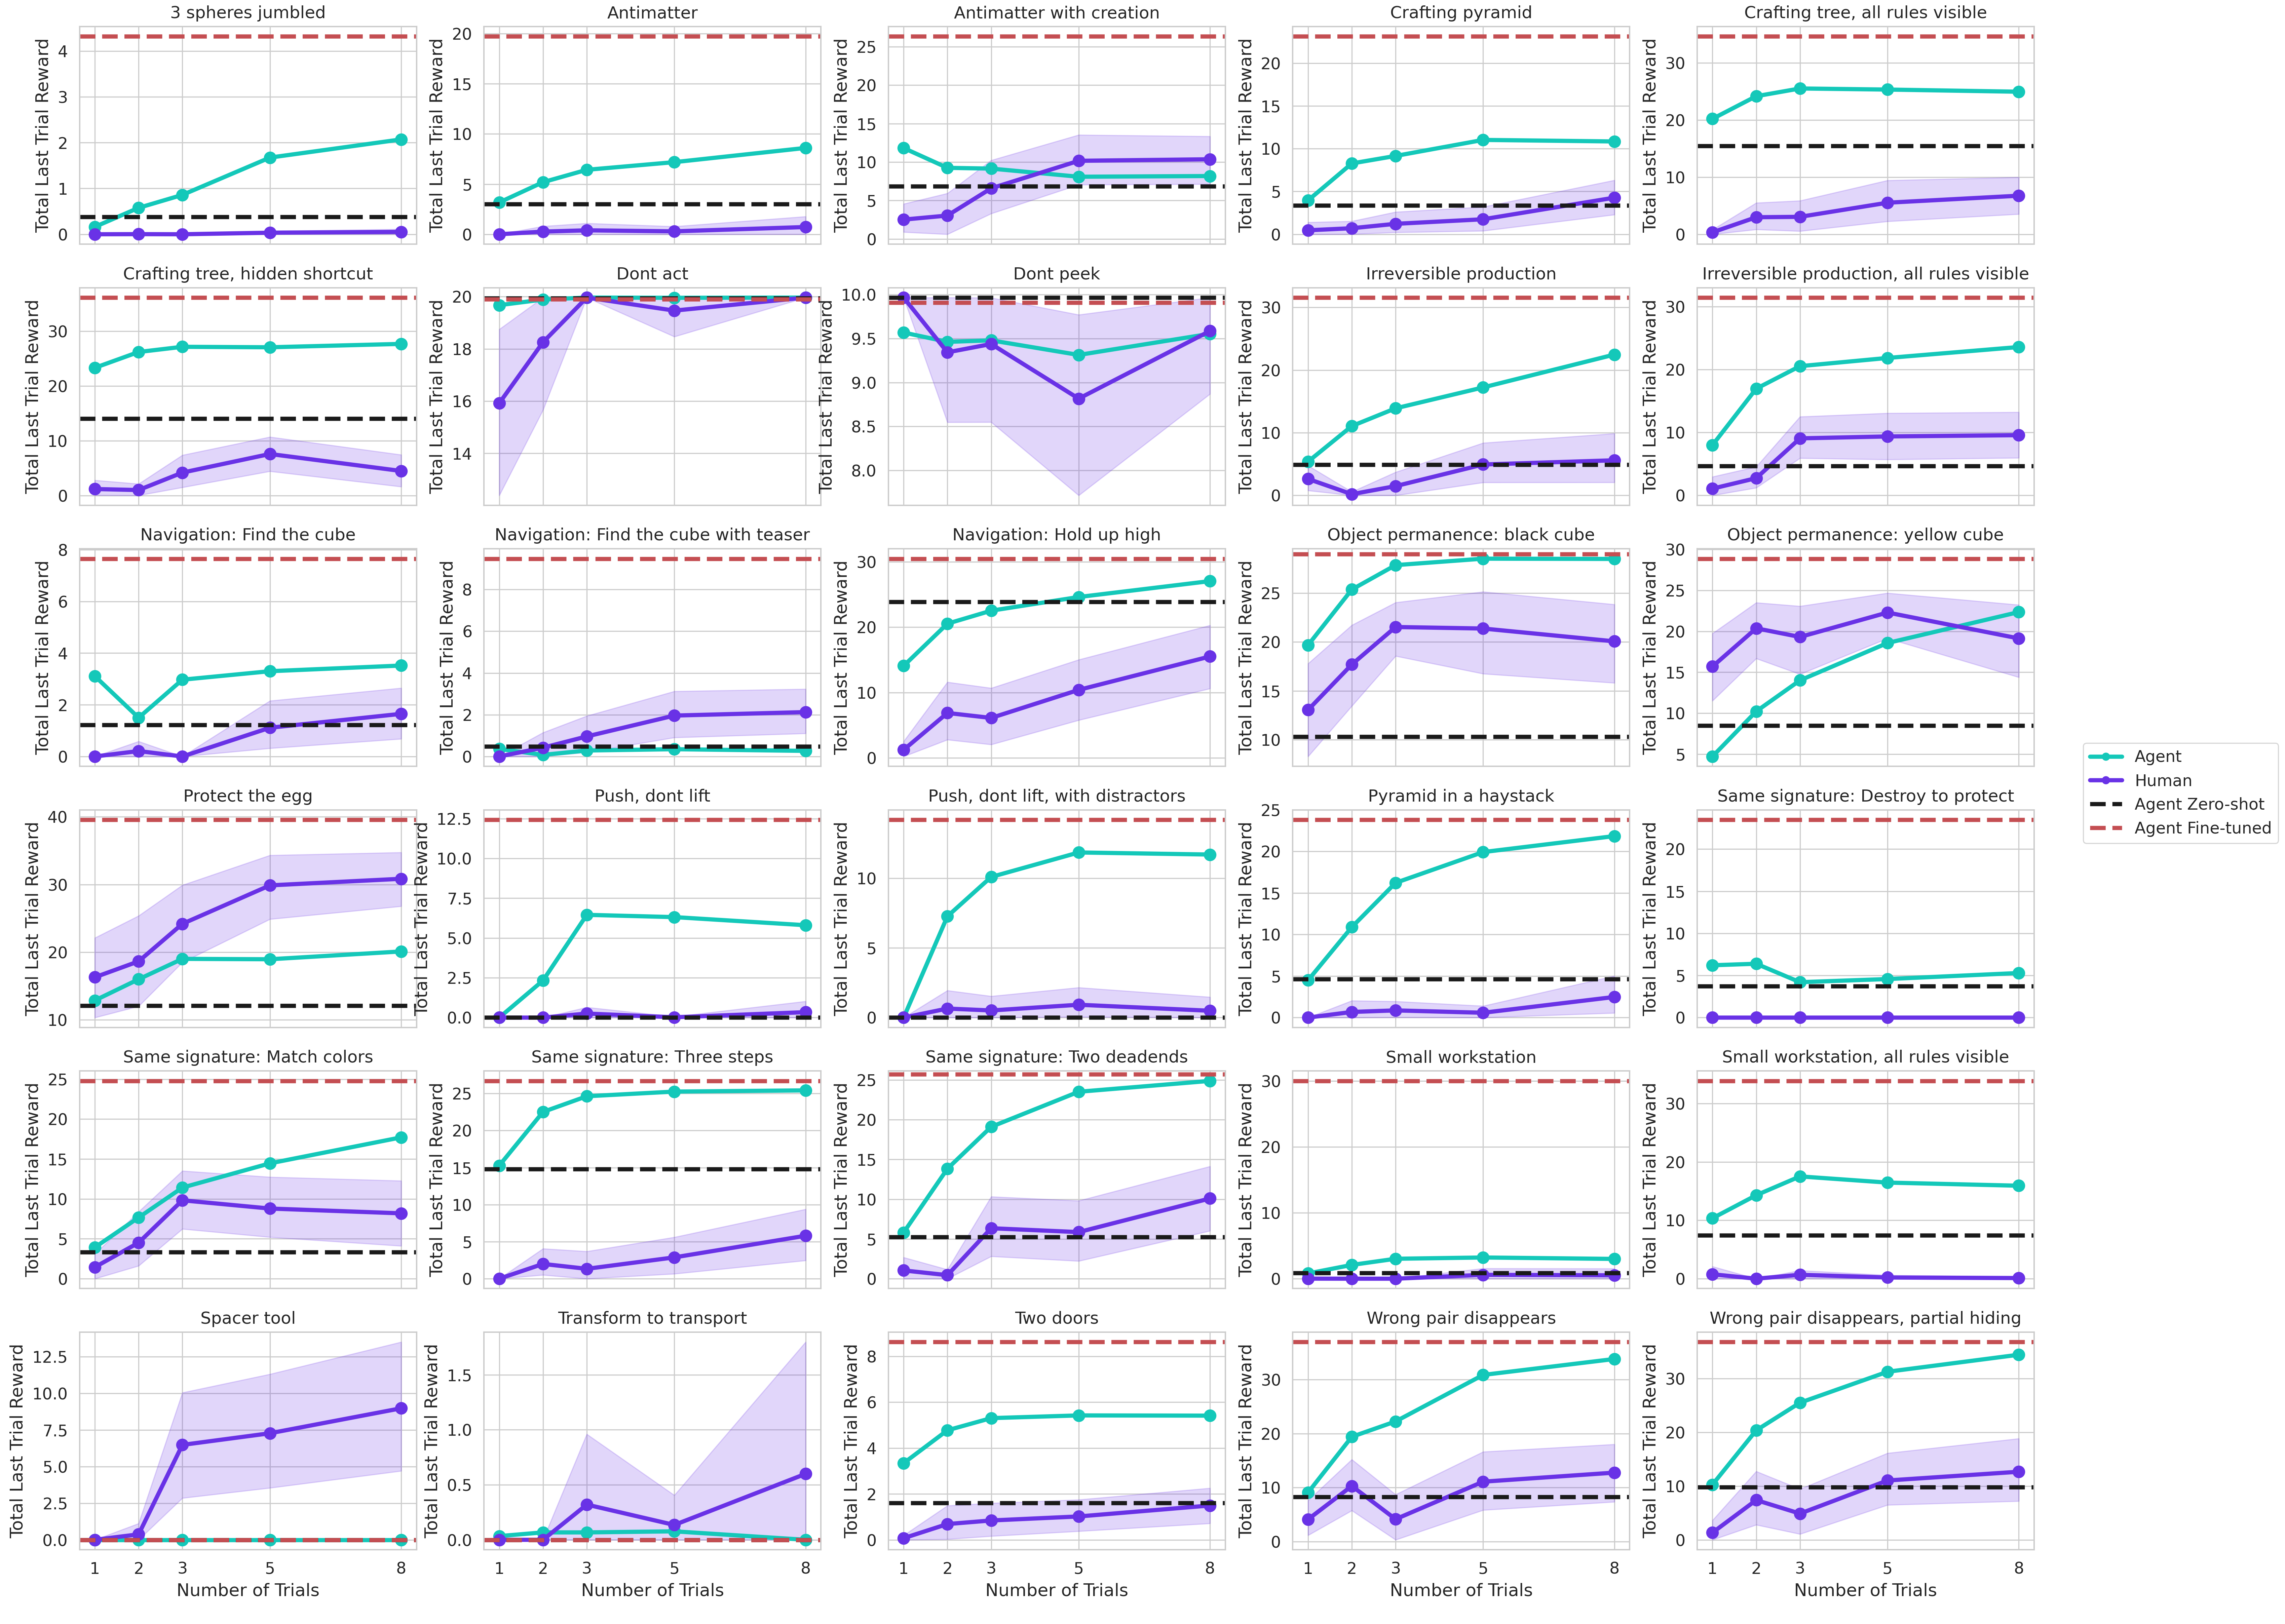
\includegraphics[width=1\linewidth]{figures/human-scale-adaptation-all-tasks.png}
    \caption{Comparison of AdA against 19 human players on each of the 30 held-out single-agent hand-authored tasks. The performance of a baseline agent trained to optimise zero-shot performance is shown as a black dashed line and indicates that AdA does not sacrifice its zero-shot generalisation to achieve adaptation. The reward of an agent fine-tuned on the hand-authored tasks is also shown as a red dashed line to provide some indication of the maximum reward achievable in a trial of each task.}
    \label{fig:human_scale_adaptation_all_tasks}
\end{figure}

In Figure \ref{fig:human_scale_adaptation_all_tasks} we show the raw last-trial total reward for humans and our agent as a function of number of trials across every one of the $30$ evaluation probe tasks. 